\chapter{ Description of the model \label{ch:numero_uno}}
\section{An invitation to Signed Distance Fields}
The use of signed distance fields (SDFs) to model organic sufaces
is a time honoured graphical technique used, for example, by Pixar
Animation Studios to model hair in \textit{The Incredibles} 
(see \cite{petrovic2005volumetric}). The idea is to define a 
function which represents the closest distance from the query point
to a point on the surface of the object that is to be represented. 
If the query point is outside, the SDF is positive,
the SDF is zero on the surface and negative inside. SDFs can be 
rendered within traditional graphics pipelines (such as OpenGL or Vulkan)
using raymarching, a method that takes place within shader programs and 
is therefore meshless. The formulae defining SDFs for common 2D and 3D 
shapes are easy to find online, see \cite{key}. Whilst the simulations 
herein are done using 2D SDFs, a quick 3D primer is given below.
\\
To motivate the primary mechanism by which cells will undergo mitosis 
in this thesis, we consider a toy example in which the equations for 
two spheres undergo a catastrophic topological change as one parameter 
changes. We start by considering the equations for two spheres which 
begin as coincident and move apart as the parameter $a$ becomes larger. 
In order to combine the first equation
\\
\begin{equation*}
    f_1(x,y,z) =  \sqrt{ (x+a)^2+y^2+z^2 } -r,
\end{equation*}
\\
with the second equation
\\
\begin{equation*}
    f_2(x,y,z) =  \sqrt{(x-a)^2+y^2+z^2 } - r,
\end{equation*}
\\
we require a smooth combination function. We construct the combined SDF
using what is called a ``union" in the graphics community 
(see \cite{fusekvisualization}). This is the pointwise minimum 
\\
\begin{equation*}
    f_{\textrm{union}}(x,y,z) = \min(f_1(x,y,z), f_2(x,y,z)).
\end{equation*}
\\
To get smooth transition between the cells as they come apart we use 
$\textrm{smoothmin}$ which is defined by a smoothness parameter $k$, as in

\begin{equation}
    \textrm{smoothmin}(x_1, x_2) = -k \log(e^{-x_1/k} + e^{-x_2/k}).
\end{equation}

As shown in Figure \ref{fig:ToyMitosis}, we have a smooth splitting of a 
cell as the parameter $a$ ranges from $0.0$ to $5.0$. Here $r$ is the
nominal sphere radii, and $k$ is a smoothing parameter. The larger $k$ 
is, the more smoothly the two curves cling to each other. We plot the 
level-$0$ surface of the smooth union SDF using MATLAB's 
\codeword{isosurface} function. 

\begin{figure}[!htb]
    \centering
    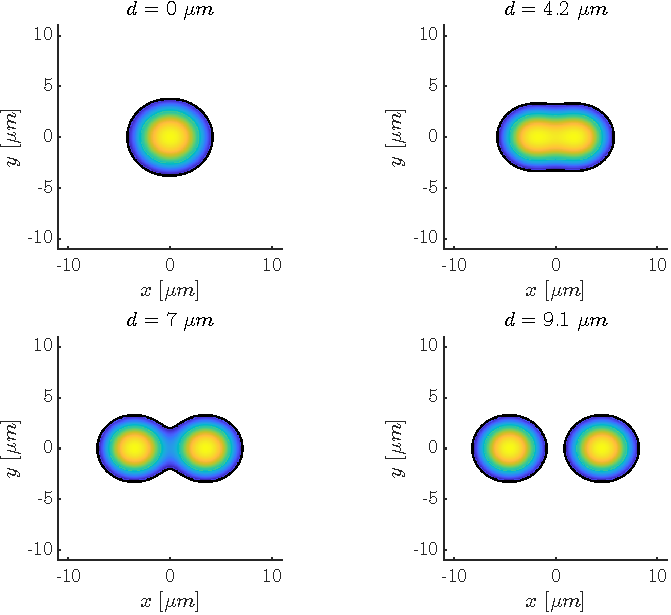
\includegraphics[width=\textwidth]{chapter1/figures/mitosisPlot.pdf}
    \caption{The separation $d$ between two ellipse shapes with $s = 0.5$ and 
    an aspect ratio of $0.9$}
    \label{fig:mitosisplot}
\end{figure}
\filbreak
It is also possible to get the intersection of two SDFs using a $\textrm{smoothmax}$ function.

\section{Modeling yeast cells with ellipses}
A signed distance field for the ellipse is used to model Baker's yeast cells.
An ellipse centered at the origin with semi-major dimension $a$ (the $x$ intercept) and
semi-minor dimension $b$ (the $y$ intercept) has an SDF given by
\begin{equation*}
    f(x,y) = \sqrt{ \left( \frac{x}{a} \right)^2 + \left( \frac{y}{b} \right)^2 } - 1.
\end{equation*}
This is not really a \textit{distance} field because it is 
dimensionless but it will still be called an SDF since it produces the 
elliptical shape all the same. Here is our ellipse.
\begin{figure}[h]
\centering
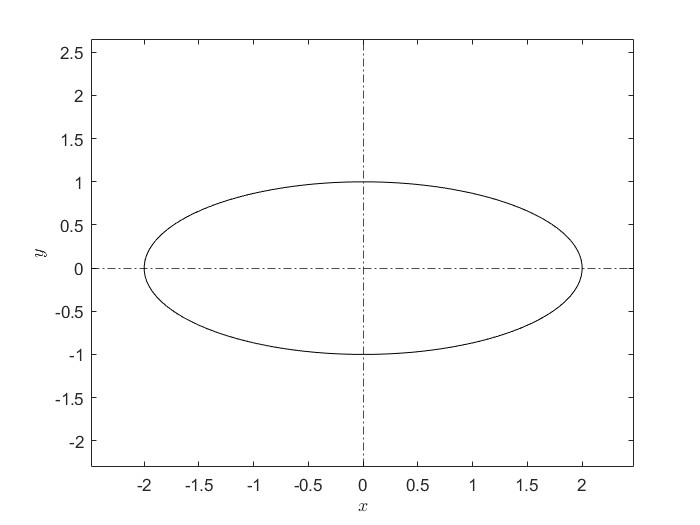
\includegraphics[width=0.5\textwidth]{chapter1/figures/ellipse_origin.jpg}
\caption{An ellipse centered at the origin with $a = 2$ and $b=1$.}
\label{fig:Ellipse_Centered}
\end{figure}
We can also translate and rotate the ellipse, using
\begin{equation*} 
    \Delta \vb{x}' = 
    \begin{bmatrix}
        \cos{\theta} & \sin{\theta} \\
        -\sin{\theta} & \cos{\theta} 
    \end{bmatrix}
    \Delta \vb{x},
\end{equation*}
where $\Delta \vb{x} = (x-x_0) \hat{\vb{i}} + (y-y_0)\hat{\vb{j}} $ and $(x_0,y_0)$ is the
center of the ellipse. We call the components of $\Delta \vb{x} = \Delta x \hat{\vb{i}} +
\Delta y \hat{\vb{j}} $ and develop the following formula
\begin{equation*}
    f(x,y) = \sqrt{ \left[\frac{ (x-x_0)\cos{\theta} + (y-y_0) \sin{\theta}}{a} \right]^2 
            +       \left[ \frac{-(x-x_0)\sin{\theta} +(y-y_0) \cos{\theta}}{b} \right]^2 } - 1.
\end{equation*}
\begin{figure}[h]
    \centering
    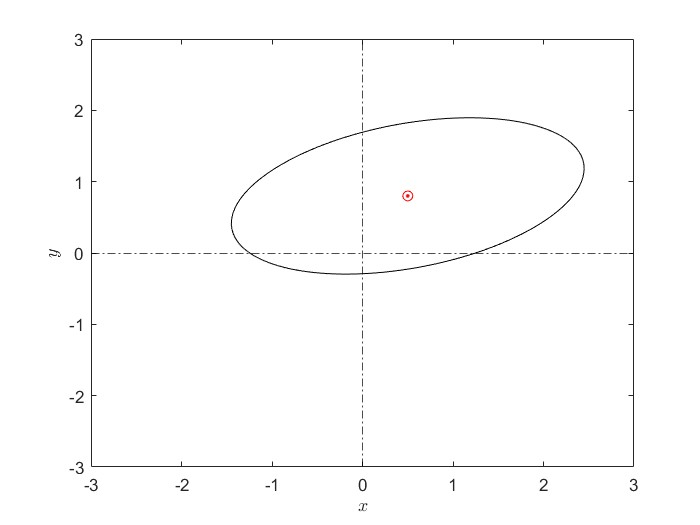
\includegraphics[width=0.5\textwidth]{chapter1/figures/ellipse_translated_rotated.jpg}
    \caption{An ellipse centered at $(0.5, 0.8)$ with $a = 2$, $b=1$ and $\theta = 15^{\circ}$.}
    \label{fig:Ellipse_Centered}
\end{figure}
\\
Cell colonies can be built up by combining the SDFs of the individual cells 
using a cumulative $\textrm{smoothmin}$. We employ the main aspect of 
$\textrm{smoothmin}$, which is that 
\begin{equation}
    \textrm{smoothmin}(f_3, \textrm{smoothmin}(f_1,f_2)) = -k \log( \sum_{j=1}^3 e^{-f_j/k}),
\end{equation}
therefore we can accumulate smoothmins easily using
\begin{equation}
    \textrm{smoothmin}(f_1, \ldots, f_N) = -k \log( \sum_{j=1}^N e^{-f_j/k}),
\end{equation}

\begin{figure}[!htb]
\centering
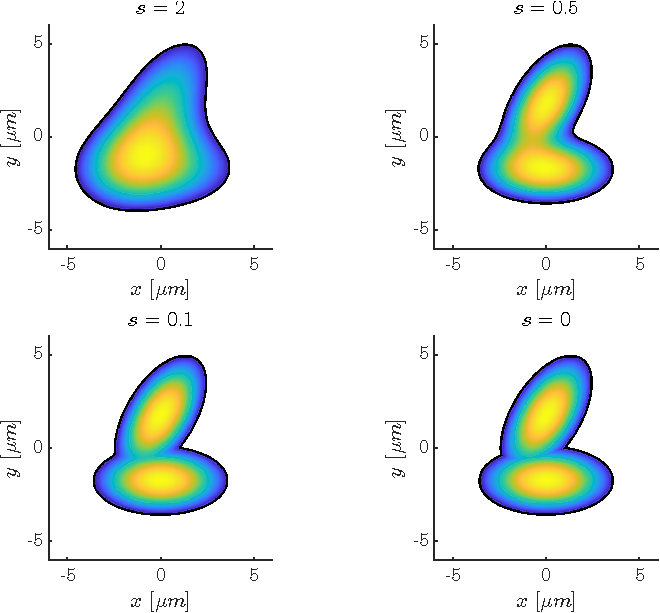
\includegraphics[width=\textwidth]{chapter1/figures/compareSmoothness.pdf}
\caption{Two ellipses blended with various values of smoothness $s$. The bottom right 
         figure is computed using standard minimum instead of smoothmin. Indeed,
         as $s \rightarrow 0$, the plot looks less smoothed across.}
\label{fig:compareSmoothness}
\end{figure}


\section{Cell colony as dynamical system}
Each cell indexed $j \in \{1, \ldots N\}$ has five pieces of data which are enough to define globally the 
SDF of the cell, namely, the center coordinates $(x_j,y_j)$, the angle of orientation $\theta_j$, 
and the semi axes dimensions $a_j, b_j$. Each piece of data will be a function of time $t$. For 
the purpose of simplicity, we model each cell as two point masses $m_1 = m_2 = m$ connected by a spring 
with stiffness $K$. The point masses are located at $\vb{r}_j^{(1)}$ and $\vb{r}_j^{(2)}$ inside the ellipse 
along the major axis and symmetrically about the ellipse center. This means that the center is given by 
\begin{equation*}
    \vb{x}_j = \frac{1}{2} \left(\vb{r}_j^{(1)} + \vb{r}_j^{(2)}\right).
\end{equation*}
Fixing the semi-minor axis $b_j$, we give the semi-major axis $a_j$ by 
\begin{equation*}
    a_j = a_0||\vb{r}_j^{(1)} - \vb{r}_j^{(2)}||.
\end{equation*}
We extract the orientation angle using a two argument inverse tangent function,
\begin{equation*}
    \theta_j = \arctan(y_j^{(2)} - y_j^{(1)},x_j^{(2)} - x_j^{(1)} )
\end{equation*}

When the number of cells is fixed, the colony dynamics is modelled
using first order EOMs with two primary forces: intracellular spring force and
and intercellular contact force to void overlap. We take the assumption that 
many authors make (include reference here) which is that inertia is negligible
due to drag effects (more on this). That is the velocity is directly
proportional to the force
\begin{equation*}
\vb{v}_j^{(i)} = \frac{1}{\eta} \vb{F}_j^{(i)},
\end{equation*}
where $i \in \{1,2\}$ and $j \in \{1, \ldots, N\}$ where $\eta$ is an expression for
the drag and $\vb{F}_j^{(i)}$ is the sum of the forces acting on the $i$-th particle of
the $j$-th cell. Overall, the simulation will be begun with $V$ vertices where $V$ is a
positive power of $2$. We map from local indices $(i,j)$ to a global index $n$ using
\begin{equation*}
    n = 2(j-1) +i,
\end{equation*}
which is called ``row major order''. We then flatten the list of $x$-coordinates and 
$y$-coordinates into one state vector $\vb{X}(t)$ given by
\begin{equation*}
    \vb{X}(t) = [x_1(t), \ldots, x_V(t), y_1(t), \ldots, y_V(t)]^T,
\end{equation*}
where $(x_n,y_n)$ is the coordinate of the $n$-th vertex for $n \in \{1,\ldots,V\}$.
Note that the change in the number of cells is simulated by removing constraints
between the vertices. At the beginning of the simulation $x_1 = \cdots = x_V$ and
$y_1 = \cdots = y_V$. The first order ordinary differential equation is phrased
in terms of a mass matrix and a force function,
\begin{equation*}
    M(t,\vb{X})\frac{d \vb{X} (t)}{dt} = f(t,\vb{X})
\end{equation*}
We start by considering the spring force acting on the $n$-th particle due to the $m$-th 
particle given $n$ and $m$ are connected by springs. This is given by $\vb{F}_{nm}^{\textrm{spring}}$ as
\begin{equation*}
    \vb{F}_{nm}^{\textrm{spring}} = 
    K(|| \vb{x}_m - \vb{x}_n|| - L_{nm}) \frac{\vb{x}_m - \vb{x}_n}{|| \vb{x}_m - \vb{x}_n||},
\end{equation*}
where $K$ is a spring constant meant to represent cell elasticity, and $L_{nm}$ is the nominal length
of the spring connecting them. There are three situations regarding edge between vertex $n$ and $m$:
either they are connected by a spring with $L_{nm}>0$, they are collocated by an equality constraint
or they are disconnected. If the two masses are collocated by an equality constraint, then the 
spring force is undefined so we must omit this. We must also omit the contact force because this 
has no sense for collocated vertices. The contact force between two disconnected vertices is given as
\begin{equation*}
    \vb{F}_{nm}^{\textrm{contact}} =
    \begin{cases} 
        C\frac{\vb{x}_m - \vb{x}_n}{|| \vb{x}_m - \vb{x}_n||}, \ \textrm{if} \ || \vb{x}_m - \vb{x}_n|| \leq d \\
        \vb{0}, \ \textrm{if} \ || \vb{x}_m - \vb{x}_n|| > d,
    \end{cases}
\end{equation*}
which is used to ensure that vertices do not overlap past a threshold distance $d$. In terms of the 
connectivity, we can encode the fact that two vertices are connected (by a spring) in an adjacency matrix
$A_{nm}$ which is equal to $1$ if they are connected and $0$ otherwise. We also introduce a second matrix
$B_{nm}$ which represents when two vertices are disconnected, i.e., $B_{nm} = 1 - A_{nm}$. A third matrix 
is introduced for collocation $C_{nm} = 1$ if $n \neq m$ and $n$ and $m$ are collocated and $0$ otherwise.
This matrix (in fact $\tilde{C}_{nm} = \sim C_{nm}$) will be used as a logical mask to filter out 
\codeword{nan} values from the force matrices. 
\\
\\
We can think of the forces (whether elastic or contact) as pairs of matrices $(F_x)_{nm}^{\textrm{spring}}$ and 
$(F_y)_{nm}^{\textrm{spring}}$ and similarly for the contact forces. We construct the $x$-component of 
the overall force vector
\begin{equation*}
    (f_x)_n = 
    \sum_{m=1}^V((F_x)^{\textrm{spring}}(A {\&}  \tilde{C}))_{nm} + 
    \sum_{m=1}^V((F_x)^{\textrm{contact}}( B  {\&}  \tilde{C}))_{nm} ,
\end{equation*}
where $A  {\&}  \tilde{C}$ are mask matrices that ensure both $A$ and not $C$ are satisfied. Similarly for the 
$y$-component,
\begin{equation*}
    (f_y)_n = 
    \sum_{m=1}^V((F_y)^{\textrm{spring}}(A {\&}  \tilde{C}))_{nm} + 
    \sum_{m=1}^V((F_y)^{\textrm{contact}}( B  {\&}  \tilde{C}))_{nm}.
\end{equation*}
The question remains: how are the mask matrices $A$, $B$ and $C$ made to change over time? Here we will do
a small illustrative example with $N=4$ cells and $V=2N = 8$ vertices. 
\\
\\
Initially all the vertices will be
collocated at the same position $(x_0,y_0)$. This means that the force vector should come out to zero because
we essentially have one particle not interacting with anything. Let us check that $A  {\&}  \tilde{C}$ and 
$B  {\&}  \tilde{C}$ both vanish. $C$ is given directly as a matrix of all ones, which says that each vertex
is constrained to every other vertex. Thus $\tilde{C} = O$ where $O$ is a  $8 \times 8$ zero matrix. 
Initially, say $A = O$ (the zero matrix) because there are no springs. Note that this immediately says that 
$B$ is a matrix of all ones. In any case, both $A  {\&}  \tilde{C} = B  {\&}  \tilde{C} = O$.
\\
\\
At some point, the effectively single particle starts growing away from its initial position. This is 
achieved by parcelling half of the vertices into one set of collocated points, and the other half
into another set of collocated points. Programmatically, we select half of the points
and translate them to a random nearby position to $(x_0,y_0)$ and modify the $C$ matrix to remove
the constraints between the first and second set,
\begin{equation*}
    C = 
    \begin{bmatrix}
    1 & 1 & 1 & 1 & 0 & 0 & 0 & 0 \\
    1 & 1 & 1 & 1 & 0 & 0 & 0 & 0 \\
    1 & 1 & 1 & 1 & 0 & 0 & 0 & 0 \\
    1 & 1 & 1 & 1 & 0 & 0 & 0 & 0 \\
    0 & 0 & 0 & 0 & 1 & 1 & 1 & 1 \\
    0 & 0 & 0 & 0 & 1 & 1 & 1 & 1 \\
    0 & 0 & 0 & 0 & 1 & 1 & 1 & 1 \\
    0 & 0 & 0 & 0 & 1 & 1 & 1 & 1 
    \end{bmatrix}
\end{equation*}
At this point, we should also set the nominal length of the springs as $L_0$ and the corresponding
matrix of lengths $L_{mn} = L_0$ (the constant matrix with value $L_0$). As it turns out, the action
of the spring pressing the vertices apart will model the geometric growth of each elliptical cell.
The $A$ matrix will be given by
\begin{equation*}
    A = 
    \begin{bmatrix}
    0 & 0 & 0 & 0 & 1 & 0 & 0 & 0 \\
    0 & 0 & 0 & 0 & 0 & 1 & 0 & 0 \\
    0 & 0 & 0 & 0 & 0 & 0 & 1 & 0 \\
    0 & 0 & 0 & 0 & 0 & 0 & 0 & 1 \\
    1 & 0 & 0 & 0 & 0 & 0 & 0 & 0 \\
    0 & 1 & 0 & 0 & 0 & 0 & 0 & 0 \\
    0 & 0 & 1 & 0 & 0 & 0 & 0 & 0 \\
    0 & 0 & 0 & 1 & 0 & 0 & 0 & 0 
    \end{bmatrix}
\end{equation*}
Now let's suppose that the vertices in one set undergo another mitosis event, splitting half of the particles
off into a third set. The new $C$ matrix, called $C'$ must reflect this change. We call 
$C(\alpha_1, \ldots, \alpha_M) = \textrm{diag}(\vb{1}_{V/2^{\alpha_1}}, \ldots,\vb{1}_{V/2^{\alpha_M}} )$ where $\vb{1}_{V/2^{\alpha_q}}$
is an all $1$'s matrix of dimension $V/2^{\alpha_q} \times V/2^{\alpha_q}$ where $q$ indexes over the powers 
of two and represents the accumulation of division events. During a mitosis event in which the $\alpha_q$-th vertex set
splits, $C(\alpha_1, \alpha_2, \ldots, \alpha_M) \rightarrow 
C(\alpha_1, \ldots, \alpha_q+1,\alpha_q+1 , \ldots\alpha_M)$. In other words, the $\alpha_q$-th matrix splits into
two matrices of half the size. In our $8 \times 8$ case, in which we divide the second vertex set, this results
in the following
\begin{equation*}
    C = 
    \begin{bmatrix}
    1 & 1 & 1 & 1 & 0 & 0 & 0 & 0 \\
    1 & 1 & 1 & 1 & 0 & 0 & 0 & 0 \\
    1 & 1 & 1 & 1 & 0 & 0 & 0 & 0 \\
    1 & 1 & 1 & 1 & 0 & 0 & 0 & 0 \\
    0 & 0 & 0 & 0 & 1 & 1 & 0 & 0 \\
    0 & 0 & 0 & 0 & 1 & 1 & 0 & 0 \\
    0 & 0 & 0 & 0 & 0 & 0 & 1 & 1 \\
    0 & 0 & 0 & 0 & 0 & 0 & 1 & 1 
    \end{bmatrix}
\end{equation*}
The new matrix $A$ is got by adding a connections between the left over smaller matrices, which
is best understood by visualising the matrix as
\begin{equation*}
    A = 
    \begin{bmatrix}
    0 & 0 & 0 & 0 & 1 & 0 & 0 & 0 \\
    0 & 0 & 0 & 0 & 0 & 1 & 0 & 0 \\
    0 & 0 & 0 & 0 & 0 & 0 & 1 & 0 \\
    0 & 0 & 0 & 0 & 0 & 0 & 0 & 1 \\
    1 & 0 & 0 & 0 & 0 & 0 & 1 & 0 \\
    0 & 1 & 0 & 0 & 0 & 0 & 0 & 1 \\
    0 & 0 & 1 & 0 & 1 & 0 & 0 & 0 \\
    0 & 0 & 0 & 1 & 0 & 1 & 0 & 0 
    \end{bmatrix}
\end{equation*}
Taking another division event on the second block, we get
\begin{equation*}
    C = 
    \begin{bmatrix}
    1 & 1 & 1 & 1 & 0 & 0 & 0 & 0 \\
    1 & 1 & 1 & 1 & 0 & 0 & 0 & 0 \\
    1 & 1 & 1 & 1 & 0 & 0 & 0 & 0 \\
    1 & 1 & 1 & 1 & 0 & 0 & 0 & 0 \\
    0 & 0 & 0 & 0 & 1 & 0 & 0 & 0 \\
    0 & 0 & 0 & 0 & 0 & 1 & 0 & 0 \\
    0 & 0 & 0 & 0 & 0 & 0 & 1 & 1 \\
    0 & 0 & 0 & 0 & 0 & 0 & 1 & 1 
    \end{bmatrix}
\end{equation*}
and 
\begin{equation*}
    A = 
    \begin{bmatrix}
    0 & 0 & 0 & 0 & 1 & 0 & 0 & 0 \\
    0 & 0 & 0 & 0 & 0 & 1 & 0 & 0 \\
    0 & 0 & 0 & 0 & 0 & 0 & 1 & 0 \\
    0 & 0 & 0 & 0 & 0 & 0 & 0 & 1 \\
    1 & 0 & 0 & 0 & 0 & 1 & 1 & 0 \\
    0 & 1 & 0 & 0 & 1 & 0 & 0 & 1 \\
    0 & 0 & 1 & 0 & 1 & 0 & 0 & 0 \\
    0 & 0 & 0 & 1 & 0 & 1 & 0 & 0 
    \end{bmatrix}
\end{equation*}



\section{Mitosis: new cells from old}
In summary, the mechanism of mitosis is a slight of hand, in the sense that
each of the nodes (two nodes per cell) are already there at the simulation
outset. The appearance of growth of the colony coincides with the nodes' progressive
dislodgement from their equality constraints with one another. Of course,
there is no reason why the model could not be modified to add nodes
that were not there to begin with, though such a model would yield
equivalent results.
\\
To interpret the model mathematically, we recall that it was desireable to have
a time parameter $t$ over which the state of the colony could vary. The main 
goal of the thesis was to demonstrate that a system, in this case a yeast colony,
which appears to acquire more dynamical variables (new coordinates for new cells for example)
could be represented by a model with a fixed number of variables which are
initially coincident.
\\
Philosophically, however, the model has some limitations. In reality, we know the growth
of fungal species such as Baker's yeast, is strongly dependent on factors such as temperature
and the environmental conditions that the colony is subjected to. This means 
that the dynamics of cell growth (the collision and interaction as well as the morphology) in 
any large colony system cannot be intrinsically defined. To put it succinctly, the dynamics of 
the colony is strongly coupled to the local environmental conditions.
\\
Does this mean that we can only model biological systems completely if all the conditions 
are incorporated? As per the discussion in the introduction about mathematical modelling,
we aim to consider the simplest viable model. This, in the case of the current work, 
is a model that has two components: a cell colony as discussed in the preceeding section, and 
a nutrient field. Indeed, their coupling determines the dynamics. 
\\
In the discussion, I will suggest ways to relax these limiting assumptions that
are outside the scope of the current work but are nonetheless interesting to consider.
\\
This model, in which the colony appears as the ``unfolding" of a network of nodes
follows on somewhat naturally from the theory of $L$-systems, in which the underlying 
discrete structure of a system is allowed to evolve deterministically based on rules
analogous to cellular automata. A criticism which has been leveled 
(find relevant paper that I read a while ago) at $L$-systems and other deterministic models
of plants for example, is what I call their intrinsic nature. That is, they effectively
rely on the assumption that a biological system's rules for developement are somehow contained
within it's structure (for instance, DNA). It is more fashionable nowadays, and indeed more 
scientifically accurate, to think of a biological system as part of a complex network 
of other organisms and environmental conditions which determine its morphology.
\\
Consider a minimalistic example of modelling the motion of a spherical ball rolling around on a table.
Two spatial paramters $x$ and $y$, together as a tuple are enough to say where it is. However, 
if the ball unexpectately falls from the table, then you would suddenly require
another parameter to describe the state of the system. The value of this classical example
is to demonstrate for $N$ particles and $M$ constraints that may suddenly change, 
we can derive rich and unexpected dynamics.
\\
The best we can hope for is that our parametrisation is somehow dense in the space
of all possible cell colony configurations that we see experimentally. There are even
some exotic cases of cellular sytems in which a single cell can have nontrivial topologies (ask Ed 
about the slime cells which optimise their topology based on nutrient). Therefore, future work 
should focus on representations of dynamic cell geometries that are as free of assumptions as
is conceivable. Once an abstract enough representation of a biological system and its environment
becomes available in the theory, one can use it to study and predict novel morphologies that appear 
in nature. Hopefully it is clear that the present work is just a suggestion of the numerous possibilities
in the area of biolgical morphology viewed in the framework of ``growing geometry''.


\section{Adding in a nutrient field}
The nutrient field is some form of glucose mixture (agar) that is assumed to be given by a reaction-diffusion 
partial differential equation. That is, the nutrient concentration $u(x,y,t)$ is given by
\begin{equation}
    \pdv{u(x,y,t)}{t} = D \left( \frac{\partial^2 u(x,y,t)}{\partial x^2} + 
                          \frac{\partial^2 u(x,y,t)}{\partial y^2} \right) - r u(x,y,t) f(x,y,t)
\end{equation}
where $f(x,y,t)$ is the microscopic biomass density of the cell colony, $D$ is a diffusion
coefficient and $r$ is a constant measuring the rate at which the cells consume nutrient.
The PDE is subjected to a Dirichlet condition, i.e
that the nutrient density vanishes at the boundary. In order to simulate the nutrient field
numerically we use a finite difference on the square grid covering the domain. This is implemented 
using a $5$-point stencil for space and a forward Euler method for time.
\begin{equation}
    \frac{u_{i,j}^{n+1} - u_{i,j}^n}{\Delta t} = 
    D \left( \frac{u_{i+1,j}^{n} - 2 u_{i,j}^n +u_{i-1,j}^n}{h^2} +
             \frac{u_{i,j+1}^{n} - 2 u_{i,j}^n +u_{i,j-1}^n}{h^2} \right)-
             r u_{i,j}^n f_{i,j}^n,
\end{equation}
where $i,j$ take on values in the interior grid points, $n$ is a positive integer time index, 
$h$ is the spatial step (same in $x$ and $y$ directions) and $\Delta t$ is the time increment. See the
figure below for an initial condition set to a sine wave product which vanishes on the boundaries.




\section{Calculating the compactness metric}
A fully grown colony will in general not be perfectly circular in shape.
 In order to measure the roundness of the colony we use the compactness metric used for 
 roundness in image processing (quote Kai use of this metric)
\begin{equation}
  C = \frac{P^2}{4 \pi A},
\end{equation}
where $C \in [1, \infty)$ is $1$ for a circle and can get to large numbers for 
highly branching shapes, $A$ is the colony area, and $P$ is the colony perimeter. 
Both of these are calculated from the formula for the microscopic cell
density which is always given by when $f(x,y,t)$ changes sign. A black and white image 
is produced at each time step using Matlab's function \codeword{bwboundaries} as per
Kai's suggestion. The area then is given by summing up the grid squares that are
inside the implicit shape givcen by $f$ and multiplying by $h^2$. The perimeter
is got by using \codeword{bwboundaries}, which outputs an array of points on the boundary
from which the Euclidean distance between neighbouring points is found and then summed over.

\begin{figure}[h]
    \centering
    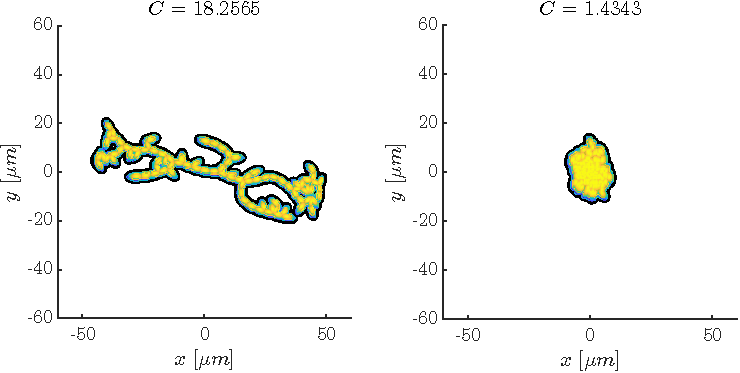
\includegraphics[width=\textwidth]{chapter1/figures/compareCompactness.pdf}
    \caption{A comparsion of high and low compactness}
    \label{fig:compatness_comparison}
\end{figure}
